\documentclass{exam}
\usepackage[utf8]{inputenc}
\usepackage{lmodern}
\usepackage{microtype}

% \usepackage[parfill]{parskip}
\usepackage[dvipsnames]{xcolor}
\usepackage{amsmath}
\usepackage{amsfonts}
\usepackage{amsthm}
\usepackage{siunitx}
\DeclareSIUnit\year{yr}
\DeclareSIUnit\foot{ft}
\DeclareSIUnit\litre{\liter}

\usepackage{skull}

\usepackage{pgfplots}
\usepgfplotslibrary{polar}
\pgfplotsset{compat=1.11}
\usepgfplotslibrary{statistics}
\usepackage{graphicx}
\usepackage{sidecap}
\sidecaptionvpos{figure}{c}
\usepackage{float}
\usepackage{gensymb}
\usepackage{tkz-euclide}
\usetkzobj{all}
\usepackage{commath}
\usepackage{hyperref}
\usepackage{enumitem}
\usepackage{wasysym}
\usepackage{multicol}
\usepackage{mathtools}
\usepackage{tcolorbox}
\usepackage{tabularx}
\usepackage[version=4]{mhchem}
\usepackage{changepage}
\usepackage{listings}
\lstset{basicstyle=\ttfamily\linespread{0.8}\small}

\renewcommand*{\thefootnote}{\fnsymbol{footnote}}

\newtheorem*{thm}{Theorem}
\newtheorem*{iden}{Identity}
\newtheorem*{lemma}{Lemma}
\newtheorem{obs}{Observation}
\theoremstyle{definition}
\newtheorem*{defn}{Definition}
\newtheorem*{ex}{Example}
\newtheorem{con}{Construction}
\newtheorem*{alg}{Algorithm}

\newtheoremstyle{break}
  {\topsep}{\topsep}%
  {\itshape}{}%
  {\bfseries}{}%
  {\newline}{}%
\theoremstyle{break}
\newtheorem*{bthm}{Theorem}

% russian integral
\usepackage{scalerel}
\DeclareMathOperator*{\rint}{\scalerel*{\rotatebox{17}{$\!\int\!$}}{\int}}

% \DeclareMathOperator*{\rint}{\int}

\pgfplotsset{vasymptote/.style={
    before end axis/.append code={
        \draw[densely dashed] ({rel axis cs:0,0} -| {axis cs:#1,0})
        -- ({rel axis cs:0,1} -| {axis cs:#1,0});
    }
}}

% \pointsinrightmargin
\boxedpoints
\pointname{}

\newcommand{\questioA}{\question[\texttt{\textbf{\color{Cerulean} A}}]}
\newcommand{\questioM}{\question[\texttt{\textbf{\color{PineGreen} M}}]}
\newcommand{\questioE}{\question[\texttt{\textbf{\color{WildStrawberry} E}}]}
\newcommand{\questioS}{\question[\texttt{\textbf{\color{Goldenrod} S}}]}
\newcommand{\questioO}{\question[\texttt{\textbf{\color{BurntOrange} O}}]}

\newcommand{\parA}{\part[\texttt{\textbf{\color{Cerulean} A}}]}
\newcommand{\parM}{\part[\texttt{\textbf{\color{PineGreen} M}}]}
\newcommand{\parE}{\part[\texttt{\textbf{\color{WildStrawberry} E}}]}
\newcommand{\parS}{\part[\texttt{\textbf{\color{Goldenrod} S}}]}
\newcommand{\parO}{\part[\texttt{\textbf{\color{BurntOrange} O}}]}

\newcommand{\subparA}{\subpart[\texttt{\textbf{\color{Cerulean} A}}]}
\newcommand{\subparM}{\subpart[\texttt{\textbf{\color{PineGreen} M}}]}
\newcommand{\subparE}{\subpart[\texttt{\textbf{\color{WildStrawberry} E}}]}
\newcommand{\subparS}{\subpart[\texttt{\textbf{\color{Goldenrod} S}}]}
\newcommand{\subparO}{\subpart[\texttt{\textbf{\color{BurntOrange} O}}]}

\newcommand{\mainHeader}[2]{\section*{NCEA Level 2 Mathematics\\#1. #2}}
\newcommand{\mainHeaderHw}[2]{\section*{NCEA Level 2 Mathematics (Homework)\\#1. #2}}
\newcommand{\seealso}[1]{\begin{center}\emph{See also #1.}\end{center}}
\newcommand{\drills}[1]{\begin{center}\emph{Drill problems: #1.}\end{center}}
\newcommand{\basedon}[1]{\begin{center}\emph{Notes largely based on #1.}\end{center}}

\begin{document}

\mainHeaderDiff{9}{Implicit Differentiation}
This week, we will take a break from applications and look at some more interesting kinds of curves. Consider
the following equations:
\begin{displaymath}
  x^2 + y^2 = 25 \text{ and } x^3 + y^4 = 5xy - 2x
\end{displaymath}
We can graph all the values $ (x,y) $ which satisfy these equations; here we have drawn the graph of the first
equation (the circle) in green and the graph of the second (the weird disconnected one) in purple.
\begin{center}
  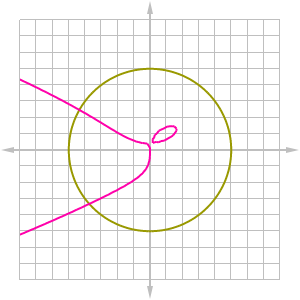
\includegraphics[width=0.3\linewidth]{implicit}
\end{center}
We can solve for the first $ y $, as $ y = \pm\sqrt{25 - x^2} $; however, the second is much harder
to solve and so we cannot find its derivative using the techniques we have studied so far. These equations
are examples of \textbf{implicit functions} of $ x $. Note that neither is a `real' function since they both fail
the vertical-line test.

The key observation here is that \textit{differentiation is an operation}, similar to addition. Just like
we can add 3 to both sides of the true equation $ 2 + 4 = 6 $ to obtain another true equation $ 2 + 3 + 4 = 3 + 6 $,
we can differentiate both sides of an equation to obtain another true equation. The only catch is that we must
remember that $ y $ is a function of $ x $ and so we must employ the chain rule.

\begin{ex}
  If $ x^2 + y^2 = 25 $, by differentiating both sides with respect to $ x $ we obtain $ 2x + \od{y}{x} 2y = 0 $ and therefore
  we have $ \od{y}{x} = -\frac{x}{y} $. Note that this depends on both $ x $ and $ y $ which makes sense:
  at $ x = 0 $, for example, we have two gradients (both of which are zero).
\end{ex}

\begin{ex}
  If $ x^3 + y^4 = 5xy - 2x $, then by differentiating both sides with respect to $ x $ we
  obtain $ 3x^2 + \od{y}{x} 4y^3 = 5y + 5x \od{y}{x} - 2 $ (being careful to use the product and chain rules in differentiating). Hence
  we have that the derivative is:
  \begin{displaymath}
    \od{y}{x} = \frac{5y - 3x^2 - 2}{4y^3 - 5x}
  \end{displaymath}
\end{ex}

\textcolor{red}{Be careful to always specify which is the variable which you are differentiating with respect to.}

\clearpage
\subsection*{Questions}
\begin{questions}
  \questioM In each case, look at the cool pictures and find $ y' $:
    \begin{multicols}{2}
    \begin{parts}
      \part $ x^3 + y^3 = 1 $
            \begin{center}
              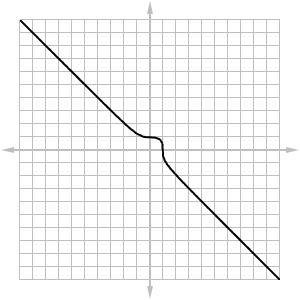
\includegraphics[width=0.6\linewidth]{implicit7}
            \end{center}
      \part $ \sin^2 y + \cos^2 x = 1 $
            \begin{center}
              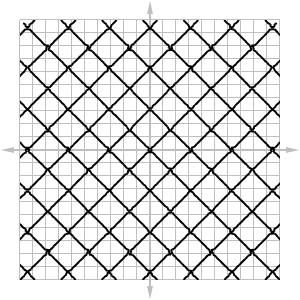
\includegraphics[width=0.6\linewidth]{implicit2}
            \end{center}
      \part $ x^3 + y^3 = 6xy $ (the folium of Descartes)
            \begin{center}
              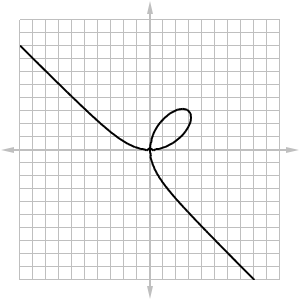
\includegraphics[width=0.6\linewidth]{folium}
            \end{center}
      \part $ y \cos x = 1 + \sin(xy) $
            \begin{center}
              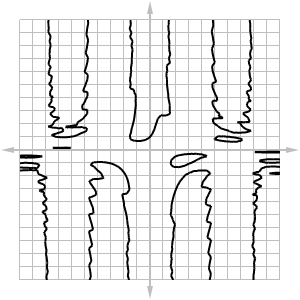
\includegraphics[width=0.6\linewidth]{implicit6}
            \end{center}
      \vfill\null
      \columnbreak
      \part $ x^2 + xy - y^2 = 4 $
            \begin{center}
              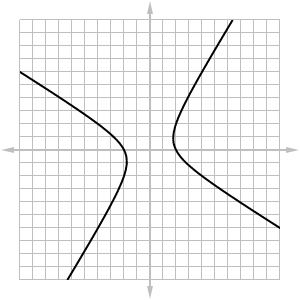
\includegraphics[width=0.6\linewidth]{implicit4}
            \end{center}
      \part $ \frac{1}{x} + \frac{1}{y} = 1 $
            \begin{center}
              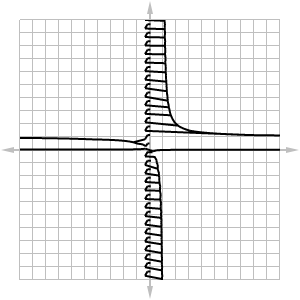
\includegraphics[width=0.6\linewidth]{implicit3}
            \end{center}
      \part $ x^2 y^2 + x \sin y = 4 $
            \begin{center}
              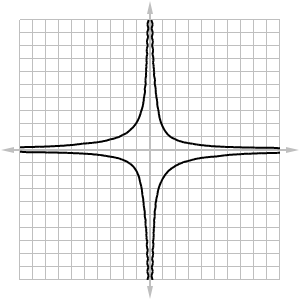
\includegraphics[width=0.6\linewidth]{implicit8}
            \end{center}
      \part $ x^4 y^2 - x^3 y + 2 x y^3 = 0 $
            \begin{center}
              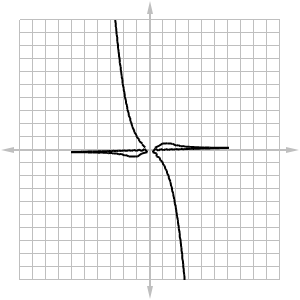
\includegraphics[width=0.6\linewidth]{implicit9}
            \end{center}
      \vfill\null
      \columnbreak
      \part $ \tan(x - y) = \frac{y}{1 + x^2} $
            \begin{center}
              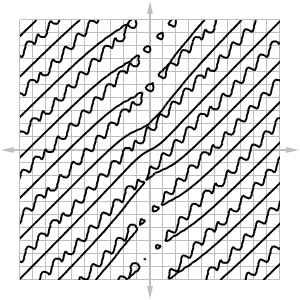
\includegraphics[width=0.6\linewidth]{implicit5}
            \end{center}
      \part $ \sin\left(\frac{x}{y}\right) = \frac{1}{2} $
            \begin{center}
              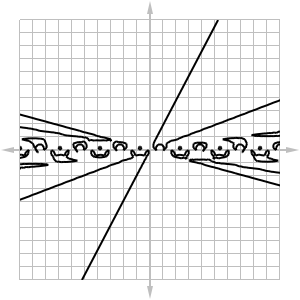
\includegraphics[width=0.6\linewidth]{implicit16}
            \end{center}
    \end{parts}
    \end{multicols}
  \questioM Consider the circle $ x^2 + y^2 = 1 $. Find the equation of the tangent to the curve at $ (\sqrt{2}, \sqrt{2}) $.
  \questioS The ellipse $ x^2 + 3y^2 = 36 $ has two tangent lines passing through the point $ (12, 3) $. Find both.
    \textit{This question is similar to one from the 2015 Scholarship paper.}
  \begin{multicols}{2}
  \questioM Find $ x' $ and $ y' $ if $ \ln(y) = \sin(xy) + \frac{x}{y} $.
            \begin{center}
              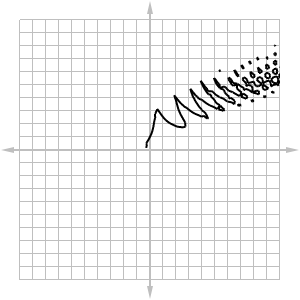
\includegraphics[width=0.6\linewidth]{implicit13}
            \end{center}
  \end{multicols}
  \begin{multicols}{2}
  \questioM Find $ y'' $ if $ x^4 + y^4 = 16$.
            \begin{center}
              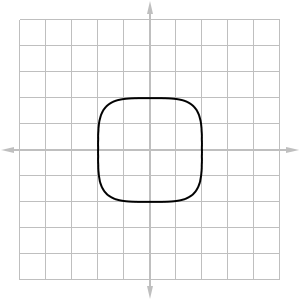
\includegraphics[width=0.6\linewidth]{implicit15}
            \end{center}
  \end{multicols}
  \begin{multicols}{2}
  \questioM If $ x^2 + xy + y^3 = 1 $, find the value of $ y''' $ at the point where $ x = 1 $.
            \begin{center}
              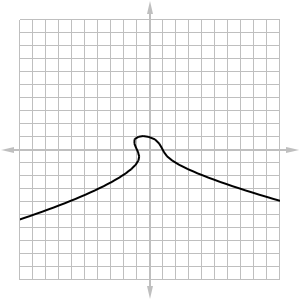
\includegraphics[width=0.6\linewidth]{implicit14}
            \end{center}
  \end{multicols}
  \begin{multicols}{2}
  \questioM Find a tangent line to the curve $ 2(x^2 + y^2)^2 = 25(x^2 - y^2) $ at the point $ (3, 1) $. This curve is known
            as a lemniscate.
            \begin{center}
              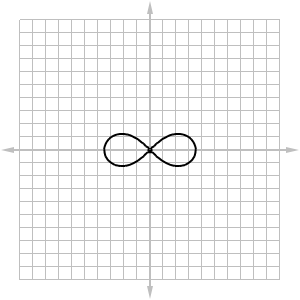
\includegraphics[width=0.6\linewidth]{lemniscate}
            \end{center}
  \end{multicols}
  \begin{multicols}{2}
  \questioM Find a tangent line to the curve $ y^2(y^2 - 4) = x^2(x^2 - 5) $ at the point $ (0, -2) $. This curve is known
            as a devil's curve.
            \begin{center}
              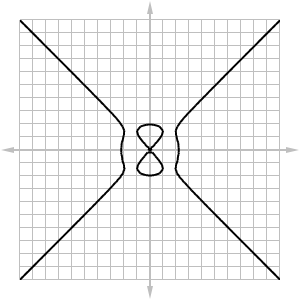
\includegraphics[width=0.6\linewidth]{devilcurve}
            \end{center}
  \end{multicols}
  \question Consider the ellipse $ x^2 - xy + y^2 = 3 $.
    \begin{parts}
      \parA Find the points where the ellipse crosses the $ x$-axis.
      \parM Show that the tangent lines of the curve at these points are parallel.
      \parE Find the maximum and minimum points of the curve.
    \end{parts}
  \questioE Consider a circle $ C $ that is tangent to $ 3x + 4y - 12 = 0 $ at $ (0, 3) $ and contains $ (2, -1) $. Set
            up equations that would determine the centre $ (h,k) $ and radius $ r $ of $ C $.
  \questioS The Bessel function of order 0, $ y = J(x) $, satisfies the differential equation
            \begin{displaymath}
              xy'' + y' + xy = 2
            \end{displaymath}
            for all values of $ x $. The value of the function at 0 is $ J(0) = 1 $.
    \begin{parts}
      \part Find $ J'(0) $.
      \part Use implicit differentiation to find $ J''(0) $.
    \end{parts}
  \clearpage
  \questioS Consider the following family of curves, known as Durer's shell curves (shown here for $ a = 2 $, $ b = 3 $):
            \begin{displaymath}
              (x^2 + xy + ax - b^2)^2 = (b^2 - x^2)(x - y + a)^2.
            \end{displaymath}
            \begin{center}
              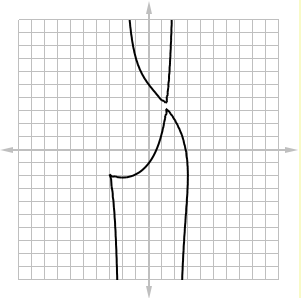
\includegraphics[width=0.3\linewidth]{durer}
            \end{center}
    \begin{parts}
      \part For which value(s) of $ b $ does the curve become a straight line?
      \part Suppose that we restrict $ a = \frac{b}{2} $. Find all non-differentiable points on the curve.
    \end{parts}
  \questioO Moving into three dimensions, let us consider the surface described by
            \begin{displaymath}
              2y(y^2 - 3x^2)(1 - z^2) + (x^2 + y^2)^2 - (9z^2 - 1)(1 - z^2) = 0.
            \end{displaymath}
            \begin{center}
              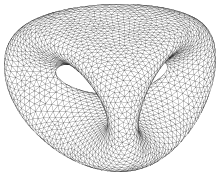
\includegraphics[width=0.3\linewidth]{impsurface}
            \end{center}
    \begin{parts}
      \part Verify that the point $ \left(1,1,\frac{1}{\sqrt{3}}\right) $ is on the surface.
      \part Find the values of $ \od{z}{x} $ and $ \od{z}{y} $ at this point (holding $ y $ and $ x $ constant, respectively). What do
            these derivatives represent?
      \part Write down the equations of the tangent lines to the surface in the $ y $ and $ x $ directions.
      \part Find an equation for the unique plane containing both tangent lines. Describe what this plane represents geometrically.
    \end{parts}
\end{questions}
\end{document}
